\documentclass[11pt,a4paper]{report}

\usepackage{fullpage}
\usepackage{fancyhdr}
\usepackage{lastpage}
\usepackage{mathtools}
\usepackage{gensymb}
\usepackage{fontspec}
\usepackage{color}
\usepackage{graphicx}
\usepackage{wrapfig}
\usepackage{tabularx}
\usepackage{hyperref}
\usepackage[french]{babel}
\usepackage{indentfirst}
\usepackage{multicol}
%\usepackage{float}
\usepackage{mdwlist}
%\usepackage{bnf}
\usepackage{listliketab}
\usepackage[export]{adjustbox}
\usepackage{subfigure}


% for languages codes
\usepackage{xcolor}
\usepackage{listings}
\renewcommand{\lstlistingname}{Extrait de code}
\lstset{basicstyle=\ttfamily,
  showstringspaces=false,
  commentstyle=\color{gray},
  keywordstyle=\color{blue}
}
% https://tex.stackexchange.com/questions/89574/language-option-supported-in-listings
\lstdefinelanguage{javascript}{
  keywords={typeof, new, true, false, catch, function, return, null, catch, switch, var, if, in, while, do, else, case, break},
  keywordstyle=\color{blue}\bfseries,
  ndkeywords={class, export, boolean, throw, implements, import, this},
  ndkeywordstyle=\color{darkgray}\bfseries,
  identifierstyle=\color{black},
  sensitive=false,
  comment=[l]{//},
  morecomment=[s]{/*}{*/},
  commentstyle=\color{gray}\ttfamily,
  stringstyle=\color{green}\ttfamily,
  morestring=[b]',
  morestring=[b]"
}


\newcommand\vartitle{Étude sur l'apprentissage par renforcement dans les jeux \\Projet de Bachelor - hepia}
\newcommand\varauthor{Federico Pfeiffer}
\newcommand\vardate{\today}

\title{\vartitle}
\author{\varauthor}
\date{\vardate}

% page layout
\pagestyle{fancyplain}
\lhead[\vartitle]{\vartitle}
\chead[]{}
\rhead[\varauthor]{\varauthor}
\lfoot[]{}
\cfoot[\thepage\ of \pageref{LastPage}]{\thepage\ of \pageref{LastPage}}
\rfoot[]{}

\renewcommand{\headrulewidth}{0.2mm}
\renewcommand{\footrulewidth}{0mm}

\setlength{\headsep}{40pt}
\setlength{\voffset}{0cm}
\setlength{\topmargin}{-1.7cm}
\setlength{\textheight}{730pt}

\setlength{\columnsep}{30pt}

\setlength{\parindent}{0mm}
\setlength{\parskip}{2mm}

% only chapters / sections / subsections are numbered 
\setcounter{secnumdepth}{2}

% only chapters / sections are in table of contents
%\setcounter{tocdepth}{1}



\hypersetup{
  hidelinks,
  pdfstartview={FitV},
  pdftitle={\vartitle},
  pdfauthor={\varauthor}
}

\begin{document}

  \begin{titlepage}
    \maketitle

    \thispagestyle{empty}

    \begin{abstract}
    // TODO
    \end{abstract}

%    \vspace{1cm}

  \end{titlepage}
  
  \newpage
  
  \tableofcontents
  
  \newpage

  \chapter{Introduction}
  
  \chapter{Théorie}
  
  \section{Notions de base}
  
  \subsection{Fonctionnement général de l'apprentissage par renforcement}
  
    \par L'apprentissage par renforcement consiste à donner une récompense à un agent lorsque ce dernier parvient à effectuer une tâche demandée, ou lorsqu'il s'en approche. De la même manière, l'agent reçoit un malus lorsque ce dernier s'éloigne de la tâche demandée. Le but de l'agent est d'obtenir un maximum de récompense. De cette manière, le comportement de l'agent est influencé par les récompenses et malus qu'il reçoit. Au fur et à mesure que l'agent effectue des actions et reçoit des récompenses/malus, ce dernier tend à renforcer un comportement menant à un maximum de récompenses, et éviter les actions menant à des malus. À noter qu'à partir de maintenant nous ne parlerons que de récompenses: un malus sera simplement traduit par une récompense négative. 
  
    \par Plus concrètement, l'agent commence par effectuer des actions aléatoires et reçoit une récompense / malus pour chaque action effectuée. Pour chaque action commise, l'agent enregistre l'état $S$ dans lequel il se trouvait, l'action effectuée, la récompense/malus reçue  et l'état $S'$ dans lequel il se retrouve suite à l'action. Si l'agent se retrouve dans un état terminal, l'environnement est réinitialisé mais l'agent garde en mémoire les actions / états / récompenses vécus. À une fréquence définie par le développeur, l'agent passe par une phase d'ajustement \textit{(training)} où il parcourt tous les actions / états / récompenses vécus de sorte à ajuster son comportement (actions choisies) lors des états futurs qu'il rencontrera, dans le but de maximiser les récompenses. 

  \subsection{Valeur d'un état}
  
    \par Jusqu'à la fin du chapitre, nous définirons le score d'un épisode par la somme des récompenses obtenues au cours des actions effectuées. Le but de l'agent est d'obtenir le meilleur score possible, et de retenir les états par lesquels il est passé afin d'obtenir ce meilleur score. (Et également de retenir les états par lesquels il est passé qu'il l'ont mené à un mauvais score). 
    
    \par Afin d'apprendre à choisir les bonnes actions à effectuer en fonction de l'état où l'agent se trouve, ce dernier a pour but d'apprendre la valeur de chaque état qu'il rencontre: un état qui le rapproche d'un meilleur score a une meilleure valeur qu'un état qui l'éloigne d'un meilleur score. 
    
    \par L'enjeu est donc de trouver une manière d'attribuer une valeur à chaque état en fonction des états qui vont suivre, afin de choisir l'action appropriée menant à un meilleur état. Prenons l'exemple (arbitraire) comprenant 2 épisodes, avec un état initial s0 \textit{(s pour state)}: 
    
    \begin{figure}[!h]
    \center
    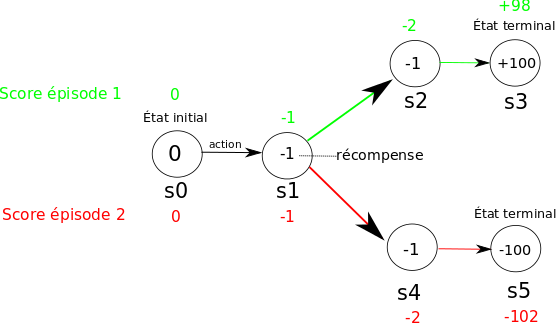
\includegraphics[scale=0.60]{ressources/introduction_function_value.png}
    \caption{Valeur d'un état: introduction 1}
    \end{figure} 
    
    \par Dans le premier épisode, l'agent commence à l'état s0 (état initial), puis choisit les actions passant par s1, s2 et s3. s3 étant un état terminal, l'épisode 1 s'arrête et l'agent obtient comme score +98 (qui est la somme des récompenses obtenues pendant son épisode). Dans le deuxième épisode, l'agent commence à l'état s0 (état initial), puis choisit les actions passant par s1, s4 et s5. s5 étant un état terminal, l'épisode 2 s'arrête et l'agent obtient un score de -102 pour le deuxième épisode. 
    
    \par Comment pourrions-nous donc attribuer une valeur à chaque état? Intuitivement, nous concluons qu'il est nécessaire d'attribuer une valeur à chaque état une fois qu'un épisode est terminé. En effet, une fois l'épisode terminé, nous pouvons évaluer chacune des actions prises par l'agent, étant donné que nous savons si les actions effectuées ont mené à l'état terminal voulu. Une première idée serait donc d'attribuer à chaque état la récompense finale auquel l'état peut mener. Si un état mène à deux récompenses différentes, nous pouvons par exemple attribuer la valeur de l'état en faisant la somme des deux récompenses auxquels l'état peut mener. 
    
    \begin{figure}[!h]
    \center
    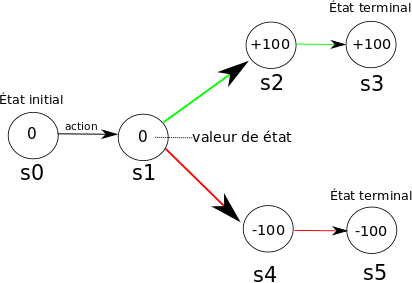
\includegraphics[scale=0.60]{ressources/introduction_function_value_2.png}
    \caption{Valeur d'un état: introduction 2}
    \end{figure}
    
    \par Après avoir effectué sa phase d'ajustement \textit{(training)} dans le but de connaître la valeur de chaque état (phase d'apprentissage), l'agent peut ensuite savoir que depuis l'état s1, il est préférable de choisir l'action menant à l'état s2, étant donné qu'un meilleur score l'attend.
    
\subsubsection{Discount factor ($\gamma$)}
  
    \par Le problème de la méthode précédente pour attribuer une valeur à un état est qu'on ne tient pas compte de la distance à laquelle se trouve la récompense finale.\\
    En prenant l'exemple suivant, il serait préférable pour l'agent de passer directement à s3 depuis s1. (L'agent a meilleur temps d'effectuer l'action qui le mène le plus rapidement à l'état menant à une forte récompense). Or, l'agent n'a pas de moyen de savoir qu'il a meilleur temps de passer directement par s3:
    
    \begin{figure}[!h]
    \center
    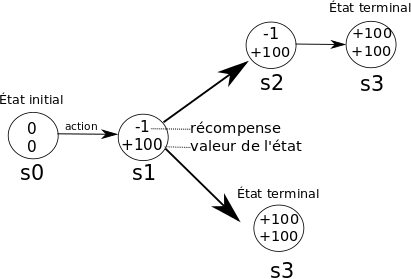
\includegraphics[scale=0.60]{ressources/introduction_function_value_3.png}
    \caption{Valeur d'un état: introduction sans discount factor}
    \end{figure}
    
    \par Une solution pour palier à ce problème est de calculer la valeur d'un état en ajoutant un coefficient nommé \textit{discount factor} $\gamma$ de cette manière: $V(s_t) = \gamma V(s_{t+1})$ avec $\gamma \in [0,1]$. En prenant $\gamma = 0.9$, on parvient à attribuer une valeur à chaque état qui inclut cette notion de distance envers la récompense la plus forte. Depuis s1, l'agent va donc tendre vers s3 directement car la valeur de s3 est plus grande que s2.
    
    \begin{figure}[!h]
    \center
    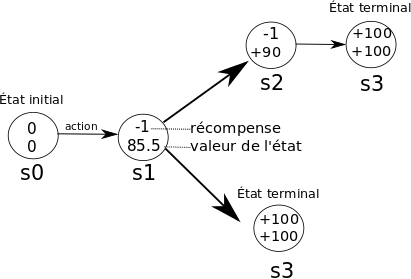
\includegraphics[scale=0.60]{ressources/introduction_function_value_4.png}
    \caption{Valeur d'un état: introduction avec discount factor}
    \end{figure} 
    
  \subsection{V(s): Équation de Bellman}
  
    \par La fonction $V(s) = \gamma V(s_{t+1})$ est incomplète. La version formelle vient de l'équation de Bellman. Elle prends en compte plusieurs notions  supplémentaires: 
    
    \par Elle prends en compte la récompense reçue à chaque état, ce qui donne \\ $V(s_t) = r + \gamma V(S_{t+1})$
    
    \par Aussi, il est possible qu'un environnement soit fait de telle sorte qu'une transition d'un état à un autre ne soit pas déterministe. Par exemple, si un agent choisit une action menant à un état $S'$, on peut imaginer que l'environnement aie un comportement aléatoire menant l'agent à un état qui n'était pas prévu par l'agent. (dans l'exemple d'une voiture autonome, le fait de voir un enfant jouer sur un trottoir n'implique pas forcément que celui-ci reste sur le trottoir). Pour un état $s_t$, il faudrait pouvoir multiplier la probabilité de se retrouver dans un état $s_{t+1}$, et recevoir une récompense $r$ après avoir fait une action $a$. En d'autres termes, pour un état $s_t$, il faut évaluer tous les états $s_{t+1}$ et toutes les récompenses $r$, et en calculer la probabilité. \\
    La fonction V(s) devient $$\sum_{s_{t+1}}\sum_rp(s_{t+1},r\ |s_t,a)\left\{r+\gamma V(s_{t+1})\right\}$$
    
    \par Enfin, il se peut que pour un certain état, l'agent aie une certaine probabilité de choisir une certaine action. (Il peut par exemple connaître la meilleur action à entreprendre, mais il a une politique d'avoir 10\% de probabilité de faire une action aléatoire dans le but d'explorer certaines actions). La fonction est alors agrémentée du terme suivant: $\sum_a\pi(a|s)$. Le $\pi$ représente la politique de l'agent.
    
    \par Ainsi, l'équation de Bellman indique que la valeur d'un état peut se calculer de la manière suivante: 
    
    $$V_\pi(s) = \sum_a\pi(a|s)\sum_{s'}\sum_rp(s',r\ |s,a)\left\{r+\gamma V_\pi(s')\right\}$$
    
    \par Le terme $\pi(a|s)$ représente la probabilité de choisir une action $a$ étant donné l'état $s$, suivant une politique $\pi$. (Dans le cas où la politique de l'agent est de choisir une action aléatoire tous les 10\% par exemple). Si l'agent a une politique visant à ne choisir que la meilleure action et que le choix de cette action n'est pas probabiliste, ce terme vaut simplement 1. De même, si l'agent n'a qu'une action possible pour un certain état $s$, le terme $\sum_a\pi(a|s)$ équivaut à $\pi(a|s)$
    
    \par Le terme $p(s',r\ |s,a)$ représente, depuis un état $s$, la probabilité de se retrouver dans l'état suivant $s'$ et de gagner la récompense $r$, ayant choisi l'action $a$. Pour connaître la valeur de l'état $s$, il faut donc pouvoir envisager tous les états $s'$ possibles, et toutes les récompenses $r$ en choisissant une action $a$. C'est pour cela que l'on "itère" en faisant la somme de tous les $p(s',r\ |s,a)$ en parcourant tous les états $s'$ possibles et toutes les récompenses $r$ possibles depuis un état $s$. D'où les deux sommes $\sum_{s'}\sum_r$ devant $p(s',r\ |s,a)$:  $\sum_{s'}\sum_rp(s',r\ |s,a)$
    
    \par L'équation de Bellman peut être lue de la manière suivante: depuis un état $s$, on itère toutes les actions possibles depuis cet état. Dans cette itération, on itère toutes les récompenses possibles et tous les états $s'$ qui découlent en choisissant l'action $a$. A chaque itération, on multiplie la probabilité $\pi(a|s)$ à la probabilité $p(s',r\ |s,a)$ et multiplie à la $\left\{r+\gamma V_\pi(s')\right\}$
    
    $$V_\pi(s) = \sum_a\pi(a|s)\sum_{s'}\sum_rp(s',r\ |s,a)\left\{r+\gamma V_\pi(s')\right\}$$
    
    \par Dans ce projet de bachelor, nous considérerons l'environnement déterministe, ce qui réduit l'équation de Bellman à ceci: 
    
    $$V_\pi(s) = \sum_a\pi(a|s)\left\{r+\gamma V_\pi(s')\right\}$$

    
  \subsection{Apprentissage par renforcement: pseudo code}
  
  \par Maintenant que nous connaissons comment attribuer une valeur à chaque état, nous pouvons imaginer un premier pseudo-code permettant à un agent d'apprendre à évoluer dans un environnement. Le problème de cette équation est qu'elle part du principe que nous connaissons tous les états et actions possibles. Il faut donc procéder de manière itérative jusqu'à ce que la valeur d'un état converge vers une valeur fixe. Nous nous arrêtons lorsque toutes les valeurs des états semblent avoir été calculées:  
  
   \begin{lstlisting}[language=python]
 
  # phase d'apprentissage
  world = new World()
  agent = new Agent()
  gamma = 0.9
  
  max_divergence = 0.1
  divergence = inf
  while divergence > max_divergence:
    for state in world.get_all_states():
      for action in world.get_possible_actions(state):
        reward, next_state = world.do_action(state, action)
        old_v = agent.V[state]
        agent.V[state] = reward + gamma * agent.V[next_state]
        divergence = max(divergence, abs(old_v-agent.V[state]))
        
  # phase une fois l'apprentissage effectué
  state = world.reset()
  while not world.is_in_terminal_state():
    action = agent.choose_action_to_best_state(state)
    state = world.do_action(action)
        
   \end{lstlisting}
  
  \par Supposer que l'on doive connaître tous les états et actions possibles pose évidemment problème dans le cas de l'apprentissage par renforcement, étant donné que l'agent doit apprendre en explorant lui-même à travers les actions qu'il entreprend. Pour des raisons de temps de calcul, nous ne souhaitons pas explorer toutes les actions possibles, mais souhaitons explorer que celles qui nous semblent nous mener à un meilleur comportement de l'agent. Heureusement, des algorithmes ont été mis en place afin de pouvoir estimer correctement la fonction de Bellman ($V(s)$) sans avoir à tout explorer, permettant ainsi à l'agent de pouvoir estimer raisonnablement la valeur de l'état dans lequel il se trouve, et choisir l'action adéquate pour maximiser son score. 
    
  \section{Algorithme Q-Learning}
  
  \subsection{Explore vs Exploit} 
  
    \par Dans la précédente section, nous avons vu un algorithme permettant d'évaluer V(s) en supposant que l'on connaisse tous les états, actions et récompenses possibles suivant l'environnement donné. Dans la majorité des cas, il n'est évidemment pas possible de connaître toutes ces valeurs à l'avance. Il convient donc d'utiliser l'agent de sorte à ce qu'il explore de lui même toutes ces différentes valeurs dans le but d'estimer correctement la fonction V(s).     
    
    \par Au fur et à mesure que l'agent explore les actions, la fonction V(s) va petit à petit atteindre une estimation correcte, et l'agent va petit à petit connaître les meilleurs états à rencontrer, ou les meilleures actions à effectuer pour chaque état. 
    
    \par Comment savoir si l'agent dispose de connaissances suffisantes pour arrêter d'explorer/tester des actions? A quel moment l'agent doit-il utiliser la connaissance qu'il dispose de V(s)? Une solution est d'effectuer une action aléatoire avec une probabilité $\epsilon$. La valeur de $\epsilon$ peut varier en fonction du temps selon ce qu'a choisit le programmeur. 
  
  \subsection{Valeur d'un état avec Q(s,a)}
  
    \par Utiliser V(s) pour attribuer une valeur à chaque état peut s'avérer limitant: on n'enregistre finalement que la valeur d'un état en fonction de l'état en question. Au lieu d'attribuer une valeur à un état, nous pourrions attribuer une valeur à un couple état/action effectué. 
    
    \par La fonction attribuant une valeur à un couple état/action s'appelle la fonction Q value, ou Q(s,a), et peut être représentée de la sorte, ressemblant fortement à V(s): 
        
    \begin{eqnarray}
      V_\pi(s) &=& \sum_a\pi(a|s)\sum_{s'}\sum_rp(s',r\ |s,a)\left\{r+\gamma V_\pi(s')\right\} \\
      Q_\pi(s,a) &=& \sum_{s'}\sum_rp(s',r\ |s,a)\left\{r+\gamma Q_\pi(s',a')\right\}
    \end{eqnarray}
    
    \par Comme indiqué plus haut, l'environnement utilisé est déterministe, ce qui permet de réduire les équations à ceci: 
    
    \begin{eqnarray}
      V_\pi(s) &=& \sum_a\pi(a|s)\left\{r+\gamma V_\pi(s')\right\} \\
      Q_\pi(s,a) &=& \left\{r+\gamma Q_\pi(s',a')\right\}
    \end{eqnarray}
    
  \subsection{Algorithme Q-Learning}
  
   \par Si nous connaissions tous les états, actions et récompenses possibles, il serait possible de définir Q(s,a) dans un environnement déterministe, de la manière suivante: 
    $$Q(s,a) = r +  \gamma Q(s',a')$$
    Or, ne connaissant pas tous les états, actions et récompenses possibles, (et ne voulant pas tous les explorer), l'idée du Q-learning est d'ajuster petit à petit Q(s,a), par une fraction $\alpha$.  
    $$Q(s,a) = old\_Q(s,a) + \alpha(new\_Q(s,a) - old\_Q(s,a))$$
    Le terme $\alpha$ est appelé "learning\_rate" est choisi arbitrairement par le développeur et est compris entre $[0,1]$. Il correspond à l'$\alpha$ utilisé lors d'un "gradient descent". 
    
    \par La méthode Q-Learning met donc Q(s,a) à jour selon la formule suivante: 
    $$Q(s,a) = Q(s,a) + \alpha(\left\{  r + \gamma Q(s', a') \right\} - Q(s,a) )$$  
    
    \par Le pseudo-code de la méthode Q-learning peut être défini de la manière suivante: 
  
   \begin{lstlisting}[language=python]
 
  # phase d'apprentissage
world = new World()
agent = new Agent()
max_episodes = 100000
gamma = 0.9
epsilon = 0.1
alpha = 0.1
  
for i in range(max_episodes):
  state = world.reset()
  while not world.game_over():
    action = agent.choose_action(state, epsilon)
    reward, next_state = world.do_action(state, action)
    a2 = agent.choose_action(next_state, epsilon)
    
    if world.game_over(): 
      agent.Q[state][action] += alpha*(reward)
    else:
      agent.Q[state][action] += alpha*(reward+gamma*agent.Q[next_state][a2])

    state = next_state
    
        
  # phase une fois l'apprentissage effectué
  state = world.reset()
  while not world.game_over():
    action = agent.choose_action(state, epsilon)
    state, _ = world.do_action(action)
        
   \end{lstlisting} 
    
  \subsection{Limitations de l'algorithme Q-Learning}
    
    \par L'inconvénient majeur de l'algorithme Q-Learning vient du fait qu'il faut pouvoir stocker la fonction Q(s,a) dans un tableau représentant chaque couple (état, action): si le fait de garder en mémoire V(s) utilise un tableau à 1 dimensions de taille équivalant à autant d'états possibles, la fonction Q(s,a) nécessite beaucoup plus de mémoire car elle doit enregistrer les valeurs dans un tableau à 2 dimensions, de taille $|S| * |A|$ cases. 
    
    \begin{figure}[!h]
    \center
    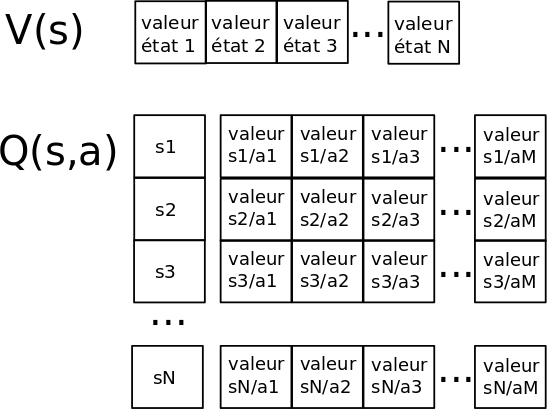
\includegraphics[scale=0.45]{ressources/v_s_vs_q_sa.png}
    \caption{Enregistrement V(s) et Q(s,a)}
    \end{figure} 
    
   \par Dans des environnements avec de nombreux (voir infinités) d'états et d'autant d'actions possibles, le stockage de la valeur de Q(s,a) devient très difficile vu la taille qu'elle représente. De plus, si l'environnement présente autant d'états et d'action possibles, l'agent va devoir effectuer beaucoup d'exploration afin d'évaluer la valeur de chaque couple (état, action), ce qui rendrait l'apprentissage extrêmement lent, voir impossible. Une solution pour palier à cet inconvénient est de remplacer le tableau Q[s][a] par un réseau neuronal. 
   
  \section{Réseaux neuronaux}
  
  \subsection{Enjeux}
  
      \par Le problème majeur des méthodes d'apprentissage par renforcement vues jusqu'ici est que lorsque l'environnement devient complexe et qu'il comporte trop d'états/actions possibles, il devient difficile (voir impossible) d'arriver à une estimation correcte que V(s) ou Q(s,a). Les réseaux neuronaux se sont révélés être de très bons estimateurs dans de nombreux champs d'applications. 
      
      \par Les réseaux de neurones sont utilisés de la manière suivante:
      
      \begin{enumerate}
      \item On crée un réseau de neurones qui a pour but d'estimer (prédire) quelque chose de précis. Au début, le réseau de neurone renvoie des réponses aléatoires. 
      \item On entraîne ce réseau de neurone en lui donnant de nombreux exemples avec la solution à estimer pour chaque exemple. (exemple d'input, solution)
      \item Au bout d'un certain nombre d'exemples donnés, le réseau de neurone s'est ajusté de sorte à pouvoir estimer (prédire) de nouveaux inputs en les estimant correctement. 
      \end{enumerate}  
      
      \par De nombreuses applications ont été trouvées pour les réseaux de neurones: on peut par exemple fournir des millier d'images comportant des tumeurs et des millier d'images ne comportant pas de tumeurs pour qu'à la fin de son apprentissage, le réseau puisse indiquer si l'image (qu'il n'a jamais vue) comporte ou ne comporte pas de tumeur. On peut également fournir un millier d'images de chiffres écrits à la main pour qu'à la fin de son apprentissage, le réseau puisse reconnaître le chiffre écrit dans une image quelconque que le réseau n'a pas encore vu. Le champ d'application est vaste: de la reconnaissance vocale à la proposition de contenu personnalisé pour Youtube ou Facebook, de nombreux domaines utilisent les réseaux neuronaux, suivant ce même principe de base. (Apprentissage, puis utilisation pour prédire quelque chose). 
      
      \par Dans le cas de l'apprentissage par renforcement, les réseaux de neurones permettent d'approximer correctement les fonctions V(s) ou Q(s,a) dans de nombreux environnements. L'utilisation d'un réseau de neurone permet les méthodes telles que le Deep Q-Learning que nous verrons dans le prochain chapitre. 
      
  \subsection{Présentation}
  
    \par Un réseau de neurones est constitué des parties suivantes: 

    \renewcommand{\labelitemi}{\textbullet}
    \begin{itemize}
    \item Une couche "d'input", représentant la couche par laquelle les données rentrent dans le réseau. Dans le cas d'images, une image est donnée à la fois. Dans le cas de l'apprentissage par renforcement, un état est donné à la fois. 
    \item Un certain nombre de couches, appelées "hidden layers". C'est dans ces couches que le réseau neuronal fait ses calculs pour effectuer une prédiction. 
    \item Une couche "d'output". C'est à travers cette couche que le résultat de la prédiction est transmise. 
    \end{itemize}    
    
    \par L'idée est que chaque neurone est relié à tous les neurones de la couche suivante, afin d'effectuer un calcul particulier à chaque couche. A la fin, la couche "output" indique le résultat de la prédiction du réseau neuronal. 
    
    \begin{figure}[!h]
    \center
    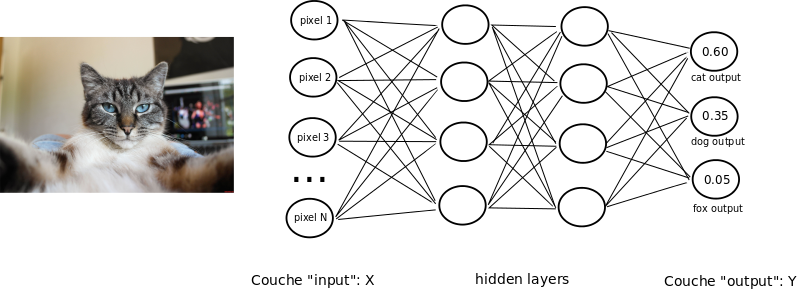
\includegraphics[scale=0.56]{ressources/nn_presentation_1.png}
    \caption{Réseau neuronal: présentation 1}
    \end{figure} 
    
    \par Dans ce premier exemple, le but du réseau neuronal est de prédire si l'image donnée dans la couche "input" est un chat, un chien, ou un renard. Le résultat de la prédiction indique que le réseau neuronal estime que l'image est à 60\% un chat, à 35\% un chien, et à 5\% un renard. Pour interpréter le résultat, on prends le neurone de sortie dont l'estimation est la plus haute: cela correspond à la sorte "chat", ce qui indique que le réseau neuronal a estimé que l'image donnée en entrée est un chat. 
    
    \begin{figure}[!h]
    \center
    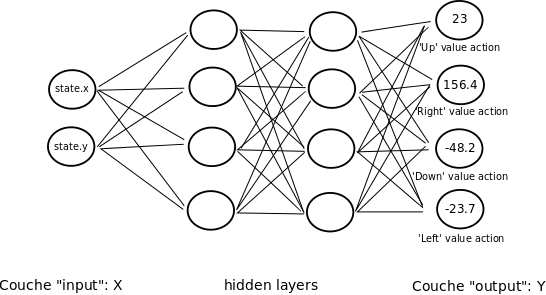
\includegraphics[scale=0.68]{ressources/nn_presentation_2.png}
    \caption{Réseau neuronal: présentation 2}
    \end{figure} 
    
    \par Dans le deuxième exemple, le but du réseau neuronal est de prédire la valeur de Q(s,a) dans l'environnement GridWorld. En input, on passe l'état dans lequel l'agent se trouve (les valeurs x et y représentant l'état). En sortie, le réseau indique l'estimation de la valeur de chaque action possible. Si l'agent ne décide pas d'effectuer une action aléatoire, l'agent prendra l'action dont la valeur est la plus haute: dans ce cas il s'agit de l'action 'Right'. 
    
  \subsection{Prédiction}

  \subsubsection{Notion de base}

    \par Pour décrire le fonctionnement d'un réseau neuronal, nous commencerons par la manière dont il effectue les prédictions. 
    
    \par Prenons l'exemple le plus simple: une valeur d'entrée (un neurone d'entrée) dont la valeur est x, une simple couche cachée d'un seul neurone contenant un poids w (weight), et une seule valeur de sortie (un seul neurone d'output) qui ne fait rien d'autre que ressortir la valeur de la couche cachée. La prédiction du neurone est calculée comme suit: 
    
    \begin{figure}[!h]
    \center
    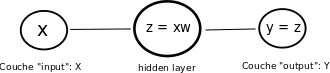
\includegraphics[scale=0.74]{ressources/nn_theory_1.png}
    \caption{Réseau neuronal: théorie 1}
    \end{figure} 
    
    \par Le but de chaque neurone caché est de prendre la valeur d'entrée, de modifier cette valeur en fonction de poids (w) (weight) que le neurone contient, et de transmettre son résultat au neurone suivant. Dans cet exemple, la prédiction vaudra: $y = z = xw$

  \subsubsection{Notation matricielle}
    
    \par Prenons maintenant le même exemple, mais avec deux valeurs en entrées. $x_1$ et $x_2$. La théorie veut que le neurone caché doit avoir 2 poids afin d'effectuer son calcul. 
    
    \begin{figure}[!h]
    \center
    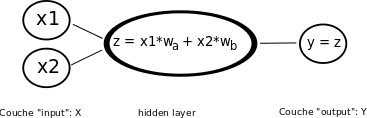
\includegraphics[scale=0.68]{ressources/nn_theory_2.png}
    \caption{Réseau neuronal: théorie 2}
    \end{figure} 
    
    \par Dans cet exemple, la prédiction vaut donc $y = z = x_1w_a + x_2w_b$
    
    \par On peut reconnaître le caractère matriciel de la prédiction et représenter la prédiction selon la notation suivante. X représente les valeurs d'entrées, W représente les poids du neurone caché, Z représente le résultat du neurone caché, et Y représente la valeur de sortie: 
    
    \begin{eqnarray}
    X &=& \begin{pmatrix} x_1 \\ x_2 \end{pmatrix} \\
    W &=&  ( w_a , w_b ) \\
    Z &=& WX  = ( w_a , w_b )\begin{pmatrix} x_1 \\ x_2 \end{pmatrix} = (x_1w_a+x_2w_b)\\
    Y &=& Z = (x_1w_a+x_2w_b)
    \end{eqnarray}
    
    \par À noter que dans la théorie qui suit, nous utiliserons la notation 'X' (majuscule) pour définir une entrée (couche input), et la notation 'Y' (majuscule) pour définir les valeurs de sortie (output). 
    
    \par Grâce à la notation matricielle, on peut maintenant imaginer un réseau avec 2 entrées et une couche de 2 neurones cachés. Comme la sortie de la couche cachée contient 2 valeurs et qu'on décide que le neurone de sortie ne fait toujours rien d'autre que de copier la sortie de la couche cachée, le neurone de sortie renverra 2 valeurs en sortie. 
    
    \begin{figure}[!h]
    \center
    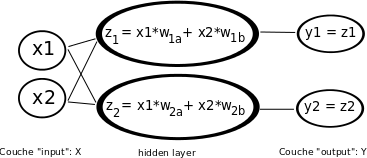
\includegraphics[scale=0.74]{ressources/nn_theory_3.png}
    \caption{Réseau neuronal: théorie 3}
    \end{figure} 
    
    \begin{eqnarray}
    X &=& \begin{pmatrix} x_1 \\ x_2 \end{pmatrix} \\
    W &=& \begin{pmatrix} w_{1a} , w_{1b} \\ w_{2a}, w_{2b} \end{pmatrix} \\
    Z &=& WX  = \begin{pmatrix} w_{1a} , w_{1b} \\ w_{2a}, w_{2b} \end{pmatrix}\begin{pmatrix} x_1 \\ x_2 \end{pmatrix} = \begin{pmatrix} w_{1a}x_1 + w_{1b}x_2 \\ w_{2a}x_1+w_{2b}x_2 \end{pmatrix} \\
    Y &=& Z = \begin{pmatrix} w_{1a}x_1 + w_{1b}x_2 \\ w_{2a}x_1+w_{2b}x_2 \end{pmatrix}
    \end{eqnarray}
    
    \par Bien entendu, si l'on souhaite n'avoir qu'une valeur en sortie, il convient de modifier le neurone de sortie de sorte à ce qu'il fasse lui aussi un calcul dont le résultat n'a qu'une matrice de 1x1. La mécanique de base reste néanmoins la même: utiliser une version matricielle pour décrire les couches et interactions entre nos neurones. De la même manière, il est possible d'ajouter plusieurs couches cachées en représentant les matrices de la bonne manière afin d'effectuer un calcul de prédiction plus complexe. 
    

  \subsubsection{Fonction d'activation}    
  
    \par Il reste encore une notion à ajouter aux réseaux neuronaux vus jusqu'ici. Les réseaux neuronaux ont été directement inspirés des vrais réseaux de neurones et de la manière dont ils fonctionnent. En termes biologiques, un neurone fait suivre une information (valeur) uniquement si le résultat de son "calcul" est supérieur à un certain seuil. En d'autres termes, un neurone ne renvoie une information que si il a suffisamment été excité. 
    
    \begin{figure}[!h]
    \center
    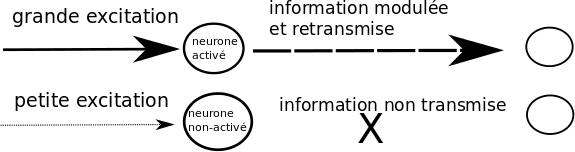
\includegraphics[scale=0.74]{ressources/nn_theory_4.png}
    \caption{Activation d'un neurone: représentation biologique}
    \end{figure} 
    
    \par Ce seuil d'activation permet aux réseaux de neurones biologiques de transmettre une information d'une manière régulée en fonction des seuils (poids) de chaque neurone. Cela permet aux réseaux de neurones biologiques d'accomplir des calculs complexes tels que la nature nous l'a montré. La notion de seuil d'excitation implique que l'intensité de chaque information transmise entre neurones doit rester comprise au sein d'un seuil biologiquement acceptable. En d'autre termes, l'intensité de l'information transmise ne peut augmenter de neurones en neurones jusqu'à atteindre une valeur trop grande, mais doit garder une intensité telle qu'un neurone puisse stopper l'information ou au contraire la retransmettre. Mathématiquement parlant, l'idée serait de garder des valeurs de sorties comprises entre [0,1]. 
    
    \par D'un point de vue complètement différent et mathématique, les opérations effectuées par les réseaux neuronaux que nous avons vues sont uniquement linéaires. Afin d'effectuer des prédictions complexes, il convient d'ajouter une notion "non-linéaire" aux opérations effectuées. Aussi, afin de pouvoir réguler facilement les poids de chaque neurone lors de la phase d'apprentissage, il convient de faire en sorte que chaque neurone renvoie une valeur de sortie comprise entre [0,1].
    
    \par Ainsi, chaque neurone passe son résultat dans une fonction non linéaire $f(x) -> [0,1]$. 
    
    \begin{figure}[!h]
    \center
    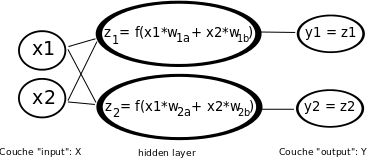
\includegraphics[scale=0.74]{ressources/nn_theory_5.png}
    \caption{Activation d'un neurone: représentation biologique}
    \end{figure} 
    
    \par L'exemple ci-dessus correspond donc à 
    
    \begin{eqnarray}
    Z &=& f(WX)  = f\left(\begin{pmatrix} w_{1a} , w_{1b} \\ w_{2a}, w_{2b} \end{pmatrix}\begin{pmatrix} x_1 \\ x_2 \end{pmatrix}\right) = f\left(\begin{pmatrix} w_{1a}x_1 + w_{1b}x_2 \\ w_{2a}x_1+w_{2b}x_2 \end{pmatrix}\right) \\
    Y &=& Z = f\left(\begin{pmatrix} w_{1a}x_1 + w_{1b}x_2 \\ w_{2a}x_1+w_{2b}x_2 \end{pmatrix}\right)
    \end{eqnarray}
    
    \par Voici les principales fonctions d'activations utilisées: 
    
    \begin{figure}[!h]
    \center
    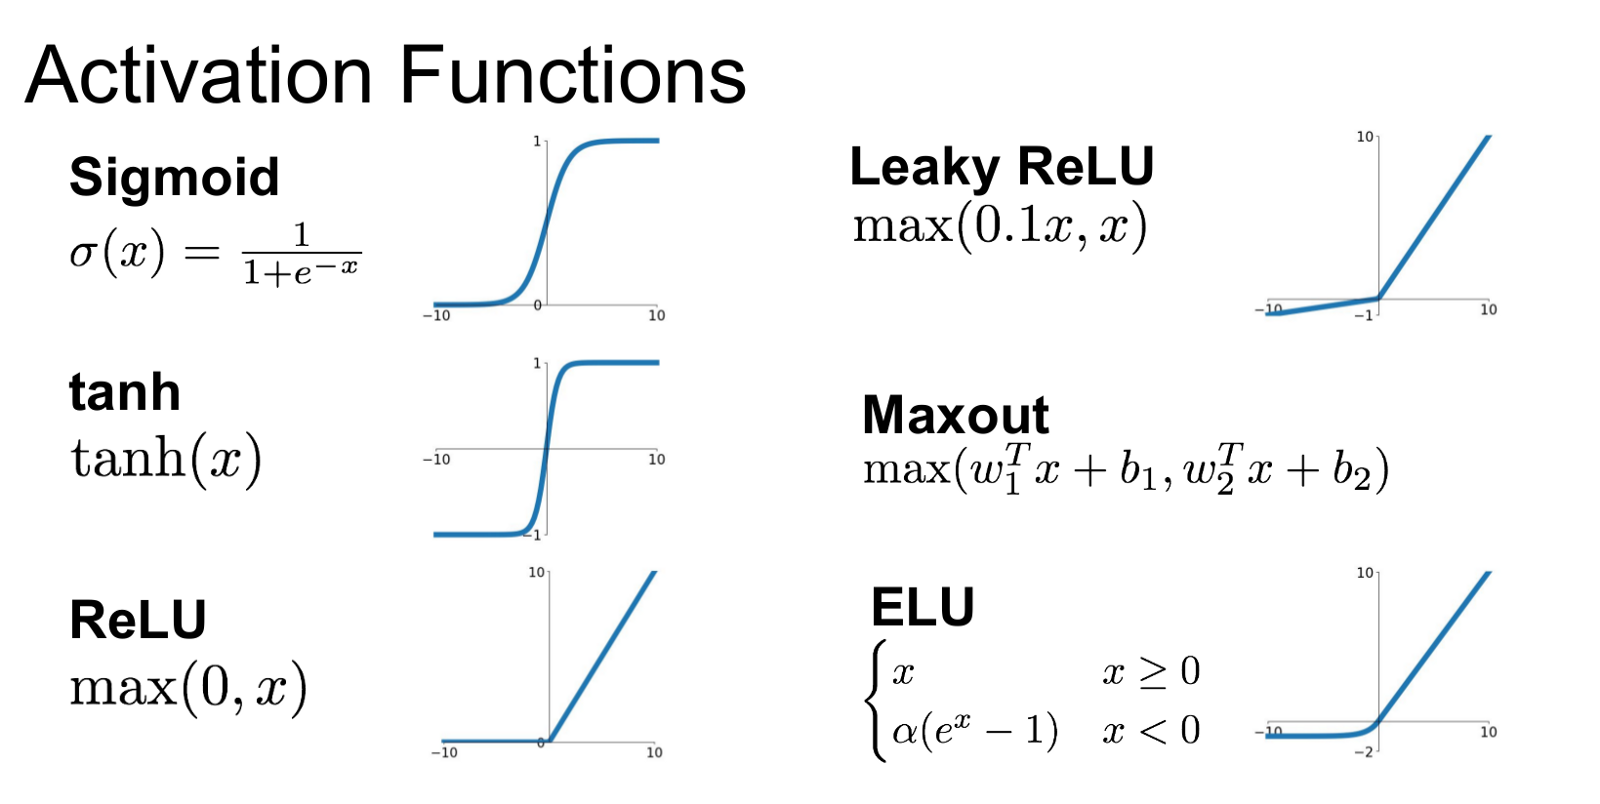
\includegraphics[scale=0.22]{ressources/activation_functions.png}
    \caption{Fonctions d'activation}
    \end{figure} 
    
    \newpage
    \par Pour terminer, le fait d'utiliser des fonctions d'activations peut comporter un problème: si un neurone émet zéro à sa sortie, il y a de fortes chances pour que le neurone suivant émette aussi 0 à sa sortie. On peut utiliser un "biais" permettant d'inhiber / stimuler l'activation d'un neurone: 
    $$Z = f(WX+b)$$
    
    \begin{figure}[!h]
    \center
    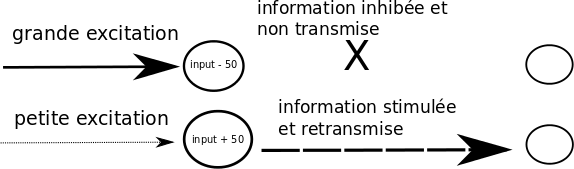
\includegraphics[scale=0.74]{ressources/nn_theory_6.png}
    \caption{Biais}
    \end{figure} 
    

    
    \par Voici donc 2 réseaux neuronaux définis mathématiquement selon toute la théorie qui a été dite: 
    
    \begin{figure}[!h]
    \center
    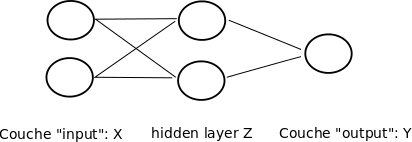
\includegraphics[scale=0.74]{ressources/nn_presentation_4.png}
    \caption{Réseau neuronal à 1 couche cachée de 2 neurones}
    \end{figure} 
    
    \begin{eqnarray}
    X &=& \begin{pmatrix} x_1 \\ x_2  \end{pmatrix}     \\
    Z &=& f\left(W_ZX+b_Z\right) = f\left(\begin{pmatrix} w_{z1a}, w_{z1b} \\ w_{z2a}, w_{z2b}\end{pmatrix}\begin{pmatrix} x_1 \\ x_2  \end{pmatrix}+\begin{pmatrix} b_{z1} \\ b_{z2}  \end{pmatrix}\right) =  \begin{pmatrix} z_1 \\ z_2  \end{pmatrix} \\
    Y &=& f_2\left( W_YZ+b_Y \right) = f_2\left( \begin{pmatrix} z_1 \\ z_2  \end{pmatrix} \begin{pmatrix} w_{ya} , w_{yb} \end{pmatrix} + b_y \right)  = (Y)
    \end{eqnarray}
    
    \newpage
    \begin{figure}[!h]
    \center
    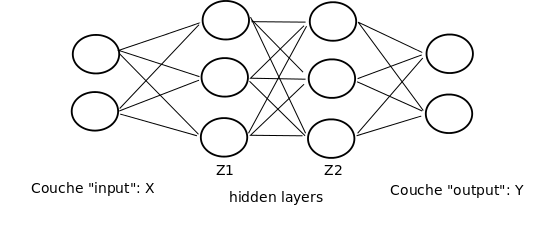
\includegraphics[scale=0.74]{ressources/nn_presentation_3.png}
    \caption{Réseau neuronal à 2 couches cachées de 3 neurones}
    \end{figure} 
    
    \begin{eqnarray}
    X &=& \begin{pmatrix} x_1 \\ x_2  \end{pmatrix}     \\
    Z1 &=& f\left(W_{z1}X+b_{z1}\right) = \begin{pmatrix} z1_{1} \\ z1_2 \\ z1_3  \end{pmatrix} \\
    Z2 &=& f_2\left(W_{z2}Z1+b_{z2}\right) = \begin{pmatrix} z2_{1} \\ z2_2 \\ z2_3  \end{pmatrix} \\
    Y &=& f_3\left( W_YZ2+b_y \right) = \begin{pmatrix} y_{1} \\ y_2  \end{pmatrix} 
    \end{eqnarray}
    

  \subsection{Apprentissage}
  
  \subsubsection{Back-propagation}
  
    \par Nous avons vu comment un neurone peut prédire un résultat Y avec des valeurs X comme entrée. Au début, tous les poids $W$ et biais $b$ de chaque neurone sont initialisés aléatoirement. Le neurone va donc prédire un résultat aléatoire. 
  
    \par L'idée de l'apprentissage est la suivante: on donne une valeur d'entrée X, dont on connaît le résultat correct de la prédiction (Target $T$). Le neurone va faire sa prédiction et sortir une valeur Y. Il faut alors ajuster chaque poids de sorte à réduire l'erreur $|Y-T|$. L'erreur peut être représentée de plusieurs manières différentes, comme par exemple $(Y - T)^2$. On représente l'erreur par une fonction $J(Y, T)$ à choix. La fonction s'appelle le "cost function". Le "phénomène" d'ajuster les poids en fonction de Y et T s'appelle Back-propagation, vu qu'un calcul va s'effectuer de la sortie vers l'intérieur du réseau de neurones. 

    \par Nous pourrions imaginer d'ajuster les poids de la manière suivante: $W = W + J(Y,T)$. Si l'erreur est grande, le poids sera "grandement" ajusté. Si l'erreur est petite, le poids sera ajusté qu'un tout petit peu. Cependant, la fonction coût $J(Y,T)$ étant positive, il faut trouver une méthode plus subtile. D'autant plus que s'il y a plusieurs couches cachées (Z1,Z2), il faudrait pouvoir ajuster les poids de Z1 uniquement en fonction de l'erreur causée par les poids de Z1, et les poids de Z2 uniquement en fonction de l'erreur causée par les poids de Z2. 

    \par La méthode utilisée pour ajuster les poids est d'utiliser la dérivée de J(Y,T). En dérivant vis à vis de chaque couche, on peut trouver l'erreur liée à chaque couche. Par conséquent, pour ajuster les poids de Z1, on effectue l'ajustement suivant: $W_{z1} = W_{z1} + \frac{dJ(Y,T)}{dW_{z1}}$. De même, pour ajuster les poids de Z2, on effectue l'ajustement suivant: $W_{z2} = W_{z2} + \frac{dJ(Y,T)}{dW_{z2}}$
  
  \subsubsection{Gradient Descent}
  
    \par Une dernière subtilité doit être ajoutée à la manière dont les poids sont ajustés. Afin d'éviter d'ajuster les poids de manière trop brutale, on ajuste (à nouveau) par une fraction $\alpha$ (learning rate). Ainsi, le méthode utilisée devient la suivante, et s'appelle la méthode du Gradient Descent: 
    
    $$W = W + \alpha \frac{dJ(Y,T)}{dW}$$
    
    \par Pour donner un exemple de calcul, prenons un cas simple, un réseau avec une couche d'entrée et une couche de sortie. (Pas de couche cachées).
    
    \begin{figure}[!h]
    \center
    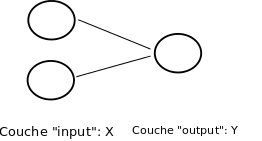
\includegraphics[scale=0.74]{ressources/nn_presentation_5.png}
    \caption{Réseau neuronal à 1 couche d'entrée et 1 couche de sortie}
    \end{figure} 
    
    \begin{eqnarray}
    Y &=& f(W_YX+b_Y) \\
    \frac{dJ}{dW_Y} &=& \frac{dJ}{dY} \frac{dY}{dW_Y} = \frac{dJ}{dY} \frac{dY}{df}\frac{df}{dW_Y}
    \end{eqnarray}
    
    \par Grâce au fait que nous travaillons avec des dérivées, l'on peut ainsi développer suffisamment pour pouvoir effectuer le calcul de $\frac{dJ}{dW_Y}$
    
    \newpage
    \par Prenons maintenant un exemple avec une couche d'entrée, une couche cachée et une couche de sortie: 
    
    \begin{figure}[!h]
    \center
    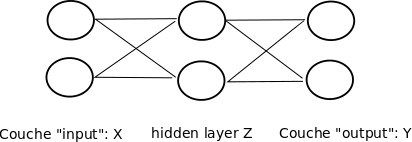
\includegraphics[scale=0.74]{ressources/nn_presentation_6.png}
    \caption{Réseau neuronal à 1 couche d'entrée, 1 couche cachée et 1 couche de sortie}
    \end{figure} 
    
    \begin{eqnarray}
    Z &=& f\left(W_ZX+b_Z\right) \\
    Y &=& f_2\left( W_YZ+b_Y \right) 
    \end{eqnarray}
    
    \par À présent, il y a deux matrices de poids à ajuster: $W_Y$ et $W_Z$. Il faut calculer leur dérivées séparément: 
    
    \begin{eqnarray}
    \frac{dJ}{dW_Y} &=& \frac{dJ}{dY} \frac{dY}{dW_Y} = \frac{dJ}{dY} \frac{dY}{df_2}\frac{df_2}{dW_Y} \\
    \frac{dJ}{dW_Z} &=& \frac{dJ}{dY} \frac{dY}{dW_Z} = \frac{dJ}{dY} \frac{dY}{df_2}\frac{df_2}{dW_Z} = \frac{dJ}{dY} \frac{dY}{df_2}\frac{df_2}{dZ}\frac{dZ}{dW_Z} = \frac{dJ}{dY} \frac{dY}{df_2}\frac{df_2}{dZ} \frac{dZ}{f_1}\frac{f_1}{dW_Z} 
    \end{eqnarray}

    \par Nous constatons (heureusement) qu'un certain schéma se répète dans le calcul des $\frac{dJ}{W_i}$, permettant ainsi le calcul des dérivées automatiquement par programmation. Plusieurs librairies fournissent cette possibilité. Pour ce travail de bachelor, la librairie TensorFlow développée par Google a été utilisée. 
    
    \par Pour conclure cette section, il est important de signaler qu'un réseau de neurone ne peut s'ajuster qu'avec un seul X et T. Il faut bien entendu répéter le calcul de back-propagation un grand nombre de fois afin d'arriver à des valeurs des poids permettant un pourcentage de prédiction correct. Une fois le réseau de neurones bien entraîné (après avoir répété la back-propagation de nombreuses fois), on peut ensuite fournir une valeur X sans connaître son résultat correct, mais en osant espérer que la prédiction sera correcte. 
  
  \subsection{Difficultés}
  
  \subsubsection{Le champ d'application des réseaux neuronaux est vaste}
  
    \par Je tiens à préciser ici que la théorie que nous avons vue dans ce chapitre ne constitue que les notions essentielles permettant appréhender correctement la suite de ce rapport. De nombreux modèles de réseaux neuronaux différèrent selon le champ d'application. Pour la reconnaissance d'images par exemple, il faut rajouter des couches de "convolution" afin de traiter les images correctement avant de faire suivre l'information dans un réseau de neurones tel que nous l'avons vu. Ces modèles de réseaux de neurones s'appellent les "convolutional neural network". De même, pour la reconnaissance de voix et prédire la phrase prononcée par un utlisateur, il faut rajouter la notion (je crois) de réseaux neuronaux récursifs, dont des sorties de certaines couches de neurones sont les entrées de couches positionnées en amont (reccurent neurals networks). 
  
  \subsubsection{Données fournies à l'apprentissage}
  
    \par Nous pouvons constater que l’efficacité d'apprentissage d'un réseau de neurones dépend fortement des données qui lui sont transmises en phase d’apprentissage. Pour donner un exemple concret, voici l'histoire d'un groupe de programmeurs ayant développé un réseau de neurones capables de décerner la différence entre un chien et un loup. Après de nombreuses sessions d'apprentissages, le réseau ne pouvait discerner un chien que lorsqu'il ne se trouvait pas entouré de neige. De même, seuls les loups étaient reconnus lorsqu'ils étaient entourés de neige. Après des semaines d'études, les développeurs se sont rendus compte que la majorité des images de loups données lors de l'apprentissage était une image d'un loup dans la neige. Les développeurs se sont ainsi rendus compte que le réseau de neurone avait appris à reconnaître la neige pour discerner un chien d'un loup. \\
  Il convient donc de faire attention à donner des données suffisamment diversifiées lors de l'apprentissage afin que celui-ci soit le plus performant possible. 
  
    \par Par ailleurs, imaginons qu'un réseau de neurones doit pouvoir classifier une valeur d'entrée entre A et B. Imaginons aussi que les seules valeurs d'entrées que nous avons pour entraîner l'agent à reconnaître 'A', soient des données X ayant pour valeurs comprises entre 100 et 1000. De même, imaginons que les données que nous avons pour entraîner l'agent à reconnaître 'B' soient des valeurs comprises entre 10 et 100. Dans ce genre de cas, il est fort probable que l'agent ne puisse pas apprendre correctement, tant les données X sont éloignées des valeurs généralement utilisées dans un réseau neuronal $X \in [0,1]$. Il convient dans la majorité des cas, d'effectuer un travail en amont afin d'uniformiser les valeurs X à fournir au réseau de neurones. Par exemple, transformer les valeurs de $[100,1000]$ à des valeurs entre $[0.1,1]$, et les valeurs entre $[10,100]$ à des valeurs comprises entre $[0.01, 0.1]$. Plusieurs stratégies existent pour cette uniformisation des données avant qu'elles soient traitées par les réseaux neuronaux. Nous ne les verrons pas dans ce rapport. 
  
  \subsubsection{Hyper-paramètres}
  
    \par Les réseaux neuronaux contiennent aussi leurs lots d'hyper-paramètres. Ne serait-ce le choix de l'architecture du réseau neuronal appelé "Modèle". Pour un même objectif, un réseau à 3 couches cachées avec 4 neurones par couche peut avoir la même performance qu'avec un réseau à 2 couches cachées contenant 2 neurones par couches.  Le choix de l'architecture a un impact significatif sur la durée d'apprentissage. 
  
    \par Une fois une architecture choisie, il y a encore beaucoup de paramètres à choisir afin de guider le réseau de neurones sur un bon apprentissage: le choix du learning rate $\alpha$, le choix des fonctions d'activations pour chaque couche, le choix de la fonction de coût J(Y,T)... De plus, d'autres méthodes alternatives à la manière d'ajuster les poids de chaque neurone existent.
  
    \par De même que dans le champ de l'apprentissage par renforcement, le choix adéquat de bons hyper-paramètres peuvent s'avérer cruciaux et seul la bonne expérience du programmeur peut mener à un bon choix de ceux-ci.   
  

  \section{Algorithme Deep Q-Learning (DQN)}
  
    \par Dans la section "Q-Learning, nous avons vu une méthode pour enseigner à un agent comment apprendre à évoluer dans un environnement donné en explorant les actions possibles. La méthode s'avère efficace lorsque l'environnement ne possède qu'une petite quantité d'états / actions possibles. Dans ces petits environnements, l'agent peut garder une copie de chaque états et actions visitées afin d'estimer correctement la fonction Q(s,a) de sorte à apprendre à savoir quelle action effectuer pour un état donné, dans le but d'effectuer un score maximal lors d'un épisode. \\ 
   Lorsque l'environnement devient plus complexe, l'espace état / actions devient beaucoup plus grand et la tâche devient presque impossible étant donné la taille du tableau Q(s,a) à garder en mémoire, et le temps nécessaire pour explorer correctement tous les couples "état / action". Les réseaux neuronaux constituent une solution  adéquate pour effectuer une estimation complexe d'un problème donné. L'enjeu du Deep Q-learning est d'utiliser les réseaux neuronaux pour effectuer une estimation suffisante de la fonction Q(s,a) sans devoir connaître / explorer l'espace complet état / actions d'un environnement donné. Un réseau neuronal peut être appelé "Deep neural network" lorsque un réseau neuronal comprends de nombreuses couches cachées; la notion de "Deep" dans "Deep Q-learning" correspond donc à appliquer la méthode Q-learning avec un réseau de neurones à plusieurs couches cachées (hidden layers). 
   
   
   \par TODO: expliquer à quoi ressemble un QNetwork.predict(): (que le réseau prédit la valeur de chaque action, donc on a un résultat de taille nb\_posible\_actions. Expliquer également qu'une action est un nombre entier entre 0 et nb\_posible\_actions. 

  \subsection{Mise à jour de la fonction Q(s,a)}
  
   \par Afin de faire fonctionner un agent avec la méthode Q-Learning utilisant un réseau neuronal pour estimer la valeur Q(s,a), il y a deux ajustements principaux à faire pour mettre à jour la fonction Q(s,a). 
  
  \subsubsection{Experience Replay}
  
  \par Comme évoqué lors du chapitre sur les réseaux neuronaux, afin qu'un réseau neuronal puisse apprendre correctement à estimer son sujet, les valeurs d'entrées X lors de la phase d'apprentissage doivent être suffisamment homogènes afin que l'apprentissage soit le plus complet possible. Or, l'idée du Q-Learning est d'ajuster Q(s,a) à chaque état parcouru de l'agent. Imaginons que l'agent commence toujours un épisode dans un même état initial: \\
  Si l'agent met à jour son réseau neuronal (Q(s,a)) à chaque état qu'il rencontre, l'apprentissage de Q(s,a) sera biaisé dans le sens où il va renforcer l'ajustement de Q(s,a) sur les premiers états (récurrents à chaque nouvel épisode), et laissera les états suivants (sporadiques) de coté pour son apprentissage. Il en résultera par exemple que l'agent connaisse les 20 premières actions à faire, mais sera incapable d'estimer correctement la suite des actions à faire. 
  
  \par Pour palier à ceci, l'idée est d'enregistrer tous les états / actions / récompenses dans une liste d'échantillons dont la longueur est définie par le programmeur. D'ici à ce que la liste d'échantillons ne soit pas pleine, l'agent ne met pas à jour la fonction Q(s,a). Si la liste est pleine, les échantillons (états / actions / récompenses) les plus vieux sont remplacés par les nouveaux échantillons rencontrés. 
  
  \par Une fois que l'on dispose d'une liste d'échantillons suffisamment grande, l'agent met à jour la fonction Q(s,a) en choisissant \textbf{aléatoirement} une \textbf{petite} partie de ces échantillons (batch). L'on par exemple mettre à jour la fonction Q(s,a) à chaque nouvel épisode, pour autant que la liste soit suffisamment grande afin de permettre de choisir \textbf{aléatoirement} un groupe d'échantillons de la liste d'échantillons. L'on peut ainsi supposer que l'agent puisse mettre à jour la fonction Q(s,a) parmi un choix d'échantillons aléatoires et suffisamment homogène. 
  
  \par Dans l'implémentation de ce dernier exercice du rapport, la liste d'échantillons états / actions / récompenses est sauvegardée dans une variable appelée \textit{experience}. Le nombre minimum d'échantillons à avoir est de 1000, et le nombre maximum à avoir est de 10'000. Lorsque l'agent possède un nombre suffisamment grand d'échantillons, ce dernier met à jour la fonction Q(s,a) en utilisant un nombre d'échantillons aléatoire (batch) de 512 échantillons. 
  
  \subsubsection{Apprentissage du réseau neuronal: Estimation Y et Target T}
  
    \par L'autre inconvénient majeur d'utiliser un réseau neuronal est que pour l’entraîner, il nous faut d'entrées X et connaître les solutions T pour chaque entrée X. En effet, le réseau neuronal ajuste ses poids lors de l'apprentissage à l'aide de la fonction J(Y, T). Or, nous ne connaissons pas T étant donné que l'idée du Q-Learning est d'explorer sans connaître son environnement. Comment choisir T étant donné que la meilleure estimation de Q(s,a) est définie par la prédiction de Q(s,a) par QNetwork? 
    
    \par En d'autres termes, si nous utilisons pour chaque X, une solution T = Y, le taux d'erreur sera de 0 et l'agent n'apprendra rien: le réseau neuronal QNetwork n'apprendra rien étant donné que la solution T correspond à la prédiction Y. 
    
    \par Une méthode qui a fait (bizarrement) ses preuves et d'avoir deux réseaux neuronaux. Le réseau pour estimer Q(s,a) (QNetwork), et un deuxième réseau pour estimer les solutions T (TNetwork). TNetwork est une copie conforme à QNetwork, à la seule différence est que TNetwork est copié de QNetwork toutes les N actions de l'agent. À l'action "0" de l'agent, QNetwork et TNetwork sont exactement les mêmes et l'apprentissage de Q(s,a) ne se fera pas. En revanche, pour les actions suivantes, QNetwork sera mis à jour et TNetwork reste le même, continuant à prédire ses valeurs T. \\
    Ainsi, Q(s,a) pourra être mise à jour étant donné que les valeurs Q(s,a) = Y de QNetwork(s) et les valeurs de TNetwork(s) = T ne fournirons pas les mêmes valeurs. 
    
    \par Bien entendu, toutes les N actions, le réseau TNetwork sera à nouveau copié depuis QNetwork car QNetwork tends à s'ajuster correctement. Dans l'implémentation du dernier exercice du rapport, TNetwork est copié depuis QNetwork toutes les 100 actions (hyper-paramètre COPY\_TARGET\_PERIOD). 
    
   \subsection{Pseudo-code de l'algorithme Deep Q-Learning} 
   
   \subsubsection{Partie principale}
   
   \par Voici un pseudo code effectuant l'algorithme Deep Q-Learning. 
   
   \begin{lstlisting}[language=python]
#*****
#MAIN
#*****
# phase d'apprentissage
world = new World()
max_episodes = 100000
gamma = 0.9
epsilon = 0.1
alpha = 0.1
QNetwork = NeuralNetwork()
TNetwork = NeuralNetwork(QNetwork)
experience = []
min_experience_size = 10000
cp_target_period = 10000
batch_size = 32
  
for i in range(max_episodes):
  state = world.reset()
  while not world.game_over():
    action = choose_action(state, epsilon, QNetwork)
    reward, next_state = world.do_action(state, action)

    experience.append((state, next_state, action, reward, game_over)) 
    if experience.length >= min_experience_size:
      train(QNetwork, TNetwork, experience, batch_size, alpha)

    if i % cp_target_period == 0:
      TNetwork.copy_from(QNetwork)
        
    state = next_state
    
        
# phase une fois l'apprentissage effectué
state = world.reset()
while not world.game_over():
  action = choose_action(state, epsilon, QNetwork)
  state, _ = world.do_action(action)
        
  \end{lstlisting} 

   \subsubsection{Fonction choose\_action()}

   \par Voici le pseudo code de la fonction choose\_action():  
  
  \begin{lstlisting}[language=python]
  
def choose_action(state, epsilon, QNetwork):
  if random() < epsilon:
    action = random_action()
  else:
    prediction = QNetwork.predict(state)
    action = argmax(prediction)
 return action
 
  \end{lstlisting} 
  
  \par Un état est représenté par un vecteur contenant les informations suffisantes pour illustrer l'état du jeu.
  \begin{lstlisting}[language=python]
  state = [agent.x, agent.y, ennemy.x, ennemy.y]
  \end{lstlisting} 
  
  \par La prédiction du réseau QNetwork prend en entrée le vecteur state, et retourne en sortie un vecteur contenant les récompenses (rewards) estimées pour chacune des actions possibles. La taille du vecteur de sortie correspond donc au nombre d'actions possibles pour l'agent. 
  
  \begin{lstlisting}[language=python]
  prediction = [ra_1, ra_2, ra_3, ra_4, ra_5] = QNetwork.predict(state)
  \end{lstlisting} 
  
  \par La fonction choose\_action() retourne l'index de la plus grande récompense estimée. Dans ce travail de bachelor, cet index équivaut à l'action choisie. Par exemple: 
  
 \begin{lstlisting}[language=python]
  prediction = [1.5, 12, -2, 1.4, 0.56] = QNetwork.predict(state)
  action = 1 = argmax(prediction)
  \end{lstlisting}
  
   \subsubsection{Fonction train()}
     
  \begin{lstlisting}[language=python]
  
def train(QNetwork, TNetwork, experience, batch_size, alpha):
  inputs = []
  choosen_actions = []
  targets = []
 
  batch = experience.pop_batch(batch_size)
  for sample in batch:
    s1, s2, w, game_over, action = sample.extract()

    inputs.append(s1)
    
    predicted_values = QNetwork.predict(s1)
    predicted_values = 0 for all values except for predicted_values[action]
    choosen_actions.append(predicted_values)
    
    target_Q_values_s2 = TNetwork.predict(s2)
    action_value = target_Q_values_s2[action]
    target = zeros(nb_posible_actions)
    target[action] = r if game_over else r + gamma * action_value
    targets.append(target)
    
  QNetwork.back_propagation(inputs, choosen_actions, targets, alpha)
    \end{lstlisting} 
  
  \par Pour entraîner le réseau QNetwork, celui-ci a besoin d'un input (vecteur représentant l'état de l'environnement), d'un vecteur représentant les valeurs qu'il a estimées (action), et les valeurs correctes qu'il aurait retourner. 
  
  \begin{lstlisting}[language=python]
  state = [agent.x, agent.y, ennemy.x, ennemy.y]
  predicted_values = [1.5, 12, -2, 1.4, 0.56]
  correct_values = target =  [2.1, 6, -2.1, 3.5, 2.21]
  \end{lstlisting} 
  
  \par Les valeurs correctes ne sont connues uniquement pour les actions qui ont été effectuées. (Pour chaque action effectuée, nous connaissons leurs récompenses et les états résultant des actions choisies. Pour chaque état, nous ne connaissons donc uniquement la valeur correcte correspondant à l'action choisie. La valeur correcte $Q(s_{visité}, a_{choisie})$ est calculée selon l'algorithme Q-Learning, en utilisant le réseau TNetwork:
  
  \begin{lstlisting}[language=python]
  target_Q_values_s2 = TNetwork.predict(s2)
  action_value = target_Q_values_s2[action]
  correct_value = target = r if game_over else r + gamma * action_value
  \end{lstlisting}   
  
  \par Or, un réseau neuronal a besoin pour s’entraîner (back-propagation) de vecteurs de la même taille que les vecteurs qu'il a en sortie. Pour entraîner le réseau uniquement sur l'action effectuée, nous créons le vecteur T (target) composé uniquement de zéros, sauf là où le réseau doit être ajusté. De même, le vecteur predicted\_values est mis à zéro partout sauf là où l'action a été effectuée. Dans cet exemple, l'action effectuée est l'action = 2. 
  
  \begin{lstlisting}[language=python]
  # avant modification
  state = [agent.x, agent.y, ennemy.x, ennemy.y] = X
  predicted_values = [1.5, 12, -2, 1.4, 0.56] = Y
  correct_values = target =  [2.1, 6, -2.1, 3.5, 2.21] = T
  
  # après modification
  state = [agent.x, agent.y, ennemy.x, ennemy.y] = X
  predicted_values = [0, 0, 0, 1.4, 0] = Y
  correct_values = target =  [0, 0, 0, 3.5, 0] = T
  \end{lstlisting} 
  
  \par De cette manière, lors du "back-propagation", l'ajustement des poids du QNetwork ne sera mis à jour que là où la dérivée $\frac{dJ(Y,T)}{dW} \neq 0$. Y = predicted\_values, et T = target.
  
  $$W = W + \alpha \frac{dJ(Y,T)}{dW}$$
  
  \par Enfin, les librairies permettent d’entraîner un réseau neuronal en lui fournissant une matrice d'inputs (X), predicted\_values (Y) et target (T). Le principe reste le même, mais cela permet d'effectuer les calculs beaucoup plus rapidement qu'en fournissant à chaque fois qu'un seul vecteur. C'est la raison pour laquelle le pseudo code entraîne le QNetwork avec des matrices (X = inputs), (Y = predicted\_values) et (T = targets). 
  
  
  \chapter{Conception}
  
  \chapter{Résultats}
  
  \chapter{Annexes}
       
\end{document}
